\documentclass[conference]{IEEEtran}
\IEEEoverridecommandlockouts
% The preceding line is only needed to identify funding in the first footnote. If that is unneeded, please comment it out.
\usepackage{cite}
\usepackage{amsmath,amssymb,amsfonts}
\usepackage{algorithmic}
\usepackage{graphicx}
\usepackage{textcomp}
\usepackage{xcolor}
\usepackage{hyperref}
\usepackage{tcolorbox}
\usepackage{listings}
\lstset{
basicstyle=\small\ttfamily,
columns=flexible,
breaklines=true
}
\usepackage{caption}
\usepackage{subcaption}
\usepackage{cellspace}
\setlength\cellspacetoplimit{4pt}
\setlength\cellspacebottomlimit{4pt}

\usepackage{tikz}
\usetikzlibrary{shapes.geometric}
\tikzstyle{startstop} = [rectangle, rounded corners, minimum width=1cm, minimum height=1cm,text centered, draw=black, fill=red!30]
\tikzstyle{io} = [trapezium, trapezium left angle=70, trapezium right angle=110, minimum width=3cm, minimum height=1cm, text centered, draw=black, fill=blue!30]
\tikzstyle{process} = [rectangle, minimum width=3cm, minimum height=1cm, text centered, draw=black, fill=orange!30]
\tikzstyle{decision} = [diamond, minimum width=3cm, minimum height=1cm, text centered, draw=black, fill=green!30]
\tikzstyle{arrow} = [thick,->,>=stealth]
\def\BibTeX{{\rm B\kern-.05em{\sc i\kern-.025em b}\kern-.08em
    T\kern-.1667em\lower.7ex\hbox{E}\kern-.125emX}}
\begin{document}

\title{EVA: A Framework for Sophisticated Text-to-Video Generation in Developing for an Extended Visual and Auditory Experience \\
{\footnotesize Batch Size of 3}
}

\author{\IEEEauthorblockN{Tyler Chan}\\
\textit{Rensselaer Polytechnic Institute}\\
Troy, NY
\and
\IEEEauthorblockN{Alan Zhang}\\
\textit{Rensselaer Polytechnic Institute}\\
Troy, NY
\and
\IEEEauthorblockN{Zhi Zheng}\\
\textit{Rensselaer Polytechnic Institute}\\
Troy, NY
}

\maketitle

\begin{abstract}

With the rise of multi-modal implementation, more artistic interpretation of ideas have been realized through text-to-image synthesis. Especially during the first lecture, where we see a story of a goat going from rags to riches selling goat cheese. Then throughout most of our class, we have explored storytelling from a single block of text. Therefore, our idea expands out storytelling, instead of an image, we want to develop a grandiose visual experience. 

With the recent breakthroughs of text-to-video synthesis, Text2Video-Zero \cite{text2vid}, there has been several advancements in the realm of text-to-video synthesis. A novel implementation of this synthesis is given at a short-form video that includes elements of the text-to-video synthesis. Then, with advancements of large language models (LLMs) like GPT-4 \cite{gpt4}, it allows us to expand a description, translating that into an entire play writer's script. All in all, the technology for a short term video given a short form description of an event is feasible.

Then, we can define this visual experience as a long-form video with relevant audio based on a specific text prompt that derives the story of the video. In short, the extended visual and auditory experience (EVA). 

\end{abstract}

\section{Introduction}

\begin{tcolorbox}
Now that some time has passed and the semester is half over, you should have a much clearer idea about your project and what will be viable to complete in the time remaining. Describe your project clearly and specify how it flows from concepts we discussed in the course. Remember that the focus should be on generative modeling (not general machine learning).
\end{tcolorbox}

\subsection{Concept of the Project}

As provided in our abstract, our motivation for our project is to explore the idea of imagination through a multidimensional lens instead of a single lens. Throughout most of the first half of the semester, we have delved deep into interpretation of generative art. With this in mind, we are looking to develop an entire story focused on a small, obscure moment. In order to accomplish this, we want to expand this moment into an entire storyboard of events and what happens throughout, like a movie script of a scene. 

Thus, what our plan for the project is: from a text, generate a script, and then utilizing this script, add on multiple short-form video and audio clips. Every script will generally have multiple scenes. These scene will include a caption and dialogue. The caption describes how the scene is acted out and the dialogue can include any auditory noises or dialogue from a particular character. For example, a possible scene for "Walter White baking bread" would contain:
\begin{lstlisting}
Caption: "Walter White inside of his bakery"
Dialogue: 
- Walter White: "My name is Walter Hartwell White and this is my bakery"
\end{lstlisting}
The opening shot represents the caption, which is the event in which the action takes place. Then the dialogue is what a particular character would say during this event. Depending on how long the audio is, multiple short-form videos will be generated with the caption that it is given. So if we have a 11 second audio clip, then we would have to generate a video of the same caption 4 different times and append those videos to make a 12 second video overall with the 11 second audio clip inserted to the video.

Of course, since we are planning to make a long-form video, we will include multiple different scenes inside of one script. For example:
\begin{lstlisting}
Script:
    - Scene 1:
        Caption: "Walter White inside of his bakery"
        Dialogue: 
        - Walter White: "My name is Walter Hartwell White and this is my bakery"
    - Scene 2:
        Caption: "Walter White opening an oven"
        Dialogue: 
        - Walter White: "All of my ingredients are fresh"
\end{lstlisting}

Finally, all of the scenes will be compiled together to make a long-form video that is directly from the storyboard, practically shot like a movie. This allows us to formulate a single text based response to an entire video that encompasses that general prompt. A good idea to get the gist of what the project is like would be to look at one of our preliminary result. That result is a good indicator of what the final product would be like for multiple different examples.

\subsection{Change in Direction}

Originally, our idea was to take style transfer in the 3D realm, and apply that to multiple different objects. However, we wanted to focus on something more generative rather than just with style transfer. Furthermore, we found difficulty replicating the papers that we mentioned earlier in our first report. Thus, we decided to change our focus on this idea.

\section{Storyboard}

\begin{tcolorbox}
Walk us through what we will see in the project. If it’s a video, what are the scenes that you need to plan and shoot/generate? If it’s a recording of a demo, what exactly will you be demonstrating? Being concrete here is meant to sharpen your planning process.
\end{tcolorbox}

The final video that we will present to the class will include the following things:
\begin{enumerate}
    \item Show the flowchart of our pipeline (see ''Fig.~\ref{fig:pipeline}'').
    \item Show an example of a prompt and the final video output.
    \item Show what the intermediate outputs of the various models are for the
    above prompt/video.
    \item Explain the underlying algorithms/models/architectures of the technologies used
    \item Show some more example videos.
    \item Finally, a live demo.
\end{enumerate}
% (Our demonstration will be the result of the product $\rightarrow$ i.e. a prompt XYZ and the result that it generated with that prompt)

\section{Related Work}

\begin{tcolorbox}
How is your project related to specific topics/algorithms/homeworks in the course? What other related work is there from the technical or artistic literature that is related to your idea, such as research papers or examples of similar effects from social media? In the case of research papers, use the proper form for citations, e.g., “This effect is similar to Radke et al. [1], who used virtual video to..." For the 6000-level I expect more academic references, not links to YouTube, but I also want each project to have a fun/creative aspect, not just a tech demo. Remember that your project should be multimodal (e.g., something involving both generative text and generative video).
\end{tcolorbox}

\subsection{Text-To-Video Generation}
The text-to-video model that we are using (Text2Video-Zero \cite{text2vid}) uses a StableDiffusion \cite{stablediffusion} model
to generate the images. This is related to the topics of using Word Embeddings, Tokens, Transformers, Attention, and CLIP that we discussed
(or going to discuss) in class for the text prompt. For the image generation a Diffusion model is used to generate images
that are conditioned on the text prompt.

\subsection{Text-To-Speech}
For the TTS, we are planning on using a VITS model to generate voice-over for the movie.
It uses a conditional VAE for inference of the spectrogram. In class we have talked about
conditional VAEs for image generation, but not for audio generation.
The demo website \cite{vits-demo} has examples of generating speech that is trained
on samples from a subject, which would be how we are generating audio that
sounds like a specific voice actor.

\subsection{LLMs}
The LLM that we are using (GPT-4 \cite{gpt4}) is related to the topics
Word Embeddings, Tokens, Transformers, and Attention that we discussed in class.

\section{Data Collection}

\begin{tcolorbox}
Data Collection. How is the data collection going? What datasets or source images/video have you already assembled and what data do you have left to collect? At this point I’m expecting that you have most of what you think you’ll need and clear plan for collecting the rest.
We have decided to not collect any data for this project due it being unnecessary.
\end{tcolorbox}

Based on our framework:
\begin{itemize}
    \item LLM: Since we are using a very complicated and well tuned model (GPT 4), we will not be fine tuning the model on any additional data. Moreover, with our group's current capability of technology, we are unable to fine-tune a LLM as good as GPT 4. In addition, we tested writing a script with captions and the output result is exactly in the format that we requested, thus we would not have any problems generating our script with GPT 4.
    % \item text-to-video: We are not generating a specific video in particular to our problem, and thus we should use
    % the pre-trained model that is the most general video model provided.
    \item text-to-video: We can fine-tune a Dreambooth \cite{dreambooth} model on a novel subject of our choice 
    (the repo for the text-to-video implementation states as such \cite{text2vid-gh}). The data that we would
    collect for this fine-tuned model would be images of our novel subject.
    \item text-to-speech: We plan to train specific voice actors for to speak the dialogue text.
    The data that we will collect would be a compendium of audio clips of the voice actor speaking
    with little to no background noise.
    % \item text-to-speech: We plan to train specific voice actors for certain results.
    % Thus, we will be gathering data for a compendium of audio from different sources that have that audio date.
    % For instance, for an audio recording for (XYZ) we will (do ABC).
    % This data has not been collected yet.
\end{itemize}

\section{Technical Approach}
\begin{tcolorbox}
Give a block/flow diagram for each main algorithm in your project, and details on
each of the sub-blocks (e.g., names/references for pre-trained standard models, network architecture and loss functions for models you trained yourself). This part should be as detailed/mathematical as you can make it. Remember, the project should have some component of hand-written code to demonstrate that you didn’t just hook together various Github repos. This is especially important at the 6000-level of the class.
\end{tcolorbox}
\begin{figure}
    \centering
    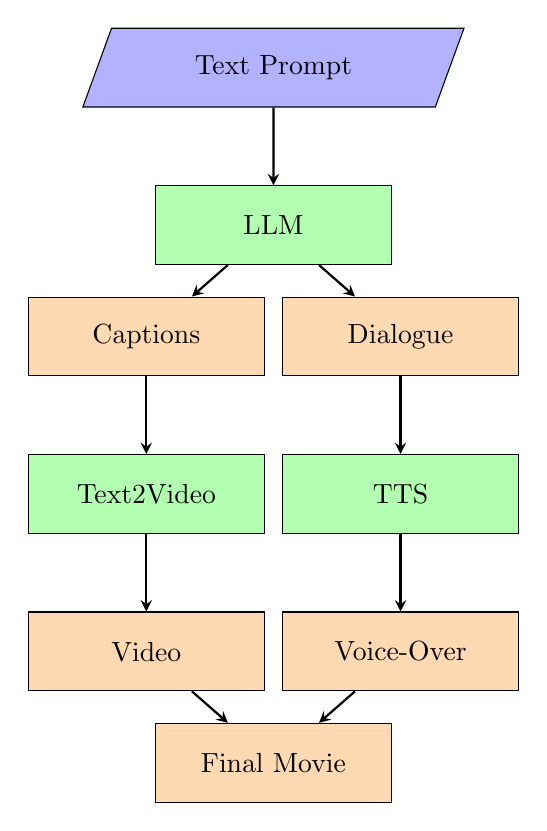
\begin{tikzpicture}[node distance=2cm]
    \node (in) [io] {Text Prompt};
    \node (LLM) [process, below of=in, fill=green!30] {LLM};
    \node (Captions) [process, below left of=LLM, xshift=-0.2cm] {Captions};
    \node (Dialogue) [process, below right of=LLM, xshift=0.2cm] {Dialogue};
    \node (Text2Video) [process, below of=Captions, fill=green!30] {Text2Video};
    \node (TTS) [process, below of=Dialogue, fill=green!30] {TTS};
    \node (Video) [process, below of=Text2Video] {Video};
    \node (Voice-Over) [process, below of=TTS] {Voice-Over};
    \node (Final Movie) [process, below left of=Voice-Over, xshift=-0.2cm] {Final Movie};
    \draw [arrow] (in) -- (LLM);
    \draw [arrow] (LLM) -- (Captions);
    \draw [arrow] (LLM) -- (Dialogue);
    \draw [arrow] (Captions) -- (Text2Video);
    \draw [arrow] (Dialogue) -- (TTS);
    \draw [arrow] (Text2Video) -- (Video);
    \draw [arrow] (TTS) -- (Voice-Over);
    \draw [arrow] (Video) -- (Final Movie);
    \draw [arrow] (Voice-Over) -- (Final Movie);
    \end{tikzpicture}
    \caption{Flowchart of Pipeline}
    \label{fig:pipeline}
\end{figure}

\subsection{Text2Video-Zero}

The problem models encountered previously with text to video synthesis is due to the unaffordant nature of large compiled datasets. Thus, a suitable, zero-shot solution is developed that requires no fine-tuning or empirical optimization. In order to do so, the model Text2Video-Zero is developed.

Text2Video-Zero is built on top of Stable Diffusion and uses cross-frame attention to keep temporal consistency and to preserve the objects in the foreground. Since it uses the image generation capabilities of Stable Diffusion, there is no training involved. To achieve this, the program introduces motion dynamics between the latent codes to maintain global scene time and changed cross-frame attention in order to preserve the appearance and identity of objects relevant to the scene.

The main issue with independently sampling latent codes from a Gaussian distribution was a random generation of images. The paper proposed that a suitable fix for this is to provide "motion dynamics" between latent codes. Motion dynamics is a method to take latent codes in a predetermined order instead of a random distribution, we define a global translation that controls the global motion of the constructed flow of a sequence. This allows us to keep temporal consistency with the diffusion process. 

Moreover, a problem that a scene can have is consistency of objects in the scene. With attention we have 
\begin{equation}
    \text{Self-Attn}(Q, K, V) = \text{Softmax}(\frac{QK^T}{\sqrt{c}})V
\end{equation}
to keep the consistency of the scene and the appearance, cross-frame attention, we can do a linear projection of the attention layers from the first frame.
\begin{equation}
    \text{Cross-Frame-Attn}(Q^k, K^{1:m}, V^{1:m}) = \text{Softmax}(\frac{Q^k(K^1)^T}{\sqrt{c}})V^1
\end{equation}

\subsection{TTS}
We recently found VITS \cite{vits} and have not looked into exactly how it works; We will include it in a later progress report.

\subsection{LLM}
OpenAI does not publish the technical details of their recent GPT models (GPT-3.5 and GPT-4) however, we can draw
parallels to the GPT-2 \cite{gpt2} models that they have published the technical details on.
The GPT \cite{gpt} architecture uses a Transformer based architecture that takes in tokens and tries to
predict the tokens that should follow the input.

\subsection{Pipeline}
Our pipeline for generating the scenes includes several different projects: an LLM \cite{gpt4}, 
Text2Video-Zero \cite{text2vid}, TTS (Text-To-Speech).

\begin{enumerate}
    \item User creates a text prompt describing for a scene or event.
    \item The LLM generates the dialogue, caption, and post processing edits for each scene.
    \item Each caption is passed to the Text2Video-Zero \cite{text2vid} model to
    get a video clip of what the caption is describing.
    \item Each dialogue is passed to a TTS program to generate a voice-over.
    \item Each video and voice-over is combined to make a final movie, and edits specified by the LLM are made to the clips.
\end{enumerate}
For clarification, refer to the flowchart of our pipeline: ''Fig.~\ref{fig:pipeline}''.

\section{Preliminary Results}
\subsection{Results}
We have created an example where the text prompt is "Walter White baking" (\href{https://www.youtube.com/watch?v=lsVTRfqRHe0}{Youtube Link}).
The clips were generated by a non-fine-tuned Text2Video-Zero \cite{text2vid} and a pre-trained model
on Walter White's voice actor on FakeYou (\href{https://fakeyou.com/about}{Link}). FakeYou was
only used to create the voice-over for this example, we plan on using open-source models like
VITS \cite{vits} for the final project. The
video clips and voice-overs were stitched together manually to 
create a prototype of what a final movie would look like.

Here is an example of the script that GPT-4 \cite{gpt4} generated in response to our prompt:
\begin{tcolorbox}
\begin{lstlisting}
    {
      "characters": [
        {"name": "Walter White"}
      ],
      "mood": "",
      "background-sound": 
        {"link":"path/to/music"},
      "script": [ 
        {"caption": "Walter White baking bread", "dialogue": [
          {"character": "Walter White", "text": "My name is Walter Hartwell White..."}
        ] }
      ]
    }
\end{lstlisting}
\end{tcolorbox}
\subsection{Reflection}
Here are some potential issues with text-to-video synthesis that we came across when generating the result and here are our potential fixes and fixes that we had:
(* denotes that it is our current solution to the problem)
\begin{itemize}
    \item text-to-video synthesis only created suitable results at a general 40-50 inferences with a capped frame count of 24. If we tried to generate more frames it would not effectively create a video (we tried 48 frames and it generated something random, that is because the model was trained to run with 24 frames). 
    \begin{itemize}
        \item we can try to extend the video by taking a frame and translating that to another video
        \item * we can just create multiple 3 second videos with the same caption if we need to extend the single clip
    \end{itemize}
    \item text-to-video synthesis can sometimes generate a setting that can be vastly different from each other. If you look at Figure ~\ref{fig:mood}, you can see that there are two videos, both of which are generated. One of them has a brighter setting and the other a dim and darker one. Thus, our problem is consistency.
    \begin{itemize}
        \item * Not completely sure, since if we have a less generalized prompt, it may be worse for the end product, but a potential solution is to add the mood to the end of the caption. So if we had "walter white baking bread" and the mood as "a bright sunny day", we can add the caption and the mood as an input. (i.e. walter white baking bread during a bright sunny day").
    \end{itemize}
\end{itemize}

\begin{figure}[h]
    \centering
    \begin{subfigure}[b]{0.5\textwidth}
        \centering
        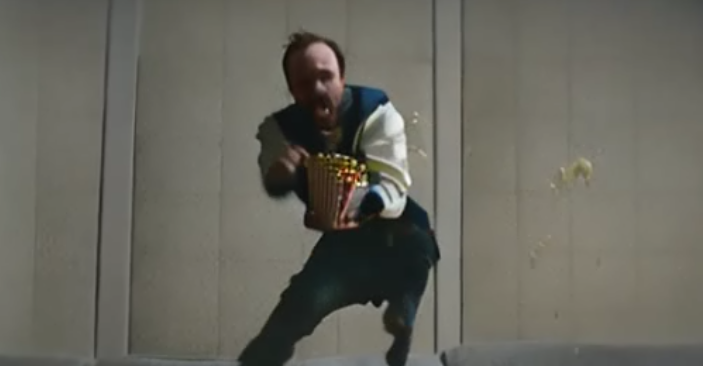
\includegraphics[width=\textwidth]{light.png}
        \caption{Jesse Pinkman throws his popcorn bowl on the floor and jumps out of his sofa with excitement}
    \end{subfigure}
    \begin{subfigure}[b]{0.5\textwidth}
        \centering
        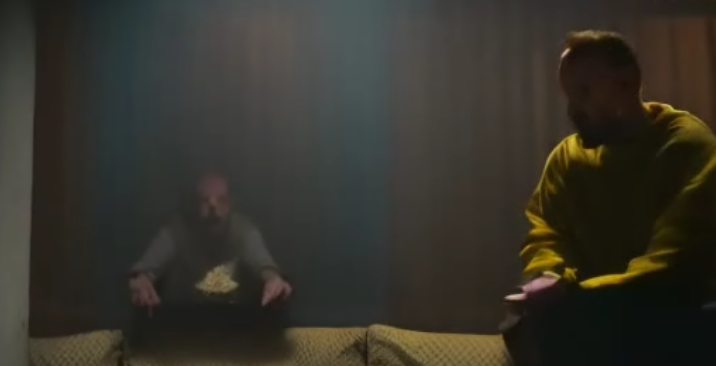
\includegraphics[width=\textwidth]{dark.png}\caption{Walter White and Jesse Pinkman sitting at a sofa both reaching for the popcorn bowl}
    \end{subfigure}
    \caption{Various moods without clarification}
    \label{fig:mood}
\end{figure}


\section{Plan for Completion and Further Work}
\subsection{Plan for Completion}
Our plan includes a progress report for each iteration of the project that needs to be accomplished, as well as the integration of the technologies that we are utilizing. These progress reports are based only for an individual tasked with an aspect of the project, and delegated to that task before a team meeting. Every report is based on when the delegated tasks are finished, and then move on to the next report.

\begin{itemize}
    \item Progress Report (1)
    \begin{itemize}
        \item The API for LLMs connected with the main script to run the pipeline
        \item A script is generated by the LLM
        \item Code to automate the video generated from the script (takes the all of the captions from the script and generates videos from the script)
        \item Train voice models (VITS) for certain characters and default characters that we will use if no special characters or models are specified.
    \end{itemize}
    \item Progress Report (2)
    \begin{itemize}
        \item An automated generation of a content (caption with characters that includes the TTS). 
        \item Automate the integration of all of the videos together, as well as the music to the background of the video.
    \end{itemize}
    \item Progress Report (3)
    \begin{itemize}
        \item Complete the entire pipeline (must take text from start and end with video at the end)
        \item Additional further work can be included if there is time to add on more
    \end{itemize}
\end{itemize}
\subsection{Further Work}
For our project, we want to completely automate the process that is in generating the scenes. We had several ideas in trying to make it so that the user may pick their favorite videos that can go into the scene as a way to cherry pick better results. Moreover, another idea that we can possibly implement if we have time is music generation. Since we have a mood given a part of the scene, we can use it to generate a background song that matches the mood of the scene. \\
\indent We will also use GPT-4 to generate general instructions for post processing each individual clip and the kind of additional visual effects that can be added, including zoom, pan, color grading, transitions effects and other various special effects. The pool of possible changes would be predetermined and we will have pre-defined functions to perform those edits. We can also incorporate user inputs during this stage should they want to customize any editing processes.

\begin{thebibliography}{00}

\bibitem{text2vid} L. Khachatryan et al., Text2Video-Zero: Text-to-Image Diffusion Models are Zero-Shot Video Generators. 2023. \href{https://arxiv.org/pdf/2303.13439.pdf}{Reference Link}

\bibitem{text2vid-gh} Picsart-AI-Research (2023) Text2Video-Zero [Source Code]. \href{https://github.com/Picsart-AI-Research/Text2Video-Zero}{Github Link}

\bibitem{stablediffusion} R. Rombach et al., High-Resolution Image Synthesis with Latent Diffusion Models. 2022. \href{https://arxiv.org/pdf/2112.10752.pdf}{Reference Link}

\bibitem{dreambooth} N. Ruiz et al., DreamBooth: Fine Tuning Text-to-Image Diffusion Models for Subject-Driven Generation. 2023. \href{https://arxiv.org/pdf/2208.12242.pdf}{Reference Link}

\bibitem{gpt4} OpenAI, GPT-4 Technical Report. 2023. \href{https://arxiv.org/pdf/2303.08774.pdf}{Reference Link}

\bibitem{gpt2} A. Radford et al., Language Models are Unsupervised Multitask Learners. 2019. \href{https://d4mucfpksywv.cloudfront.net/better-language-models/language_models_are_unsupervised_multitask_learners.pdf}{Reference Link}

\bibitem{gpt} A. Radford et al., Improving Language Understanding by Generative Pre-Training. 2018. \href{https://s3-us-west-2.amazonaws.com/openai-assets/research-covers/language-unsupervised/language_understanding_paper.pdf}{Reference Link}

\bibitem{vits} J. Kim, J. Kong, and J. Son, Conditional Variational Autoencoder with Adversarial Learning for End-to-End Text-to-Speech. 2021.\href{https://arxiv.org/pdf/2106.06103.pdf}{Reference Link}

\bibitem{vits-demo} jaywalnut310 (2021) Vits-Demo [Source Code]. \href{https://jaywalnut310.github.io/vits-demo/index.html}{Github Link}

%\bibitem{dreamfusion} G. B. Poole, A. Jain, J. T. Barron, and B. Mildenhall, DreamFusion: Text-to-3D using 2D Diffusion. 2022. \href{https://arxiv.org/pdf/2209.14988.pdf}{Reference Link}
%\bibitem{prolificdreamer} Z. Wang et al., ProlificDreamer: High-Fidelity and Diverse Text-to-3D Generation with Variational Score Distillation. 2023.\href{https://arxiv.org/pdf/2209.14988.pdf}{Reference Link}
%\bibitem{nerf} B. Mildenhall et al. NeRF: Representing Scenes as Neural Radiance Fields for View Synthesis. 2020. \href{https://arxiv.org/pdf/2003.08934.pdf}{Reference Link}
%\bibitem{nerf2mesh} T. Jiaxiang et al., Delicate Textured Mesh Recovery from NeRF via Adaptive Surface Refinement. 2022. \href{https://arxiv.org/pdf/2303.02091.pdf}{Reference Link}

\end{thebibliography}

\end{document}
